\section{梯度方法}
\label{sec:opt-smooth-gradient-methods}

上一节说明，在$L$光滑的目标上，步长$1/L$的负梯度步一定下降。本节研究只用梯度和少量历史，能把这个保证推进到什么程度。四个小节固定同一个问题和同一类评价标准，依次改变一个要素：先只改变步长的选法（固定步长或线搜索），再改变度量位移的坐标（预条件），最后让更新带上前几步的记忆（重球法与Nesterov方法）。每一种改变都写清算法维护的状态、一轮更新、接受或停止规则、所需条件与每轮代价。

\subsection{梯度下降与线搜索}
\label{sec:opt-smooth-gd-linesearch}

\term{梯度下降}（gradient descent）从初值出发，反复沿负梯度走一步：
\begin{equation}
\label{eq:opt-smooth-gd}
  \bm x^{(t+1)}=\bm x^{(t)}-\eta^{(t)}\nabla f(\bm x^{(t)}),\qquad t=0,1,2,\dots
\end{equation}
算法的状态只有当前点；每轮计算一次梯度，若要监控目标或使用线搜索，再计算若干次函数值。下面先研究已知光滑常数时的固定步长，再研究常数未知时怎样让函数值本身决定步长。

\begin{algorithm}[固定步长梯度下降]
\label{alg:opt-smooth-gd}
\begin{algorithmic}[1]
\Require 可微目标$f$，初值$\bm x^{(0)}$，步长$\eta>0$，梯度容差$\varepsilon>0$，最大轮数$T$
\Ensure 返回点$\hat{\bm x}$
\State $\hat{\bm x}\gets\bm x^{(0)}$
\For{$t=0,1,\dots,T-1$}
  \State $\bm g^{(t)}\gets\nabla f(\bm x^{(t)})$
  \If{$\lVert\bm g^{(t)}\rVert_2<\lVert\nabla f(\hat{\bm x})\rVert_2$} \State $\hat{\bm x}\gets\bm x^{(t)}$ \Comment{记录梯度最小的已访问点}\EndIf
  \If{$\lVert\bm g^{(t)}\rVert_2\leq\varepsilon$} \State \Return $\bm x^{(t)}$ \EndIf
  \State $\bm x^{(t+1)}\gets\bm x^{(t)}-\eta\,\bm g^{(t)}$
\EndFor
\State \Return $\hat{\bm x}$（凸目标也可返回最后一点$\bm x^{(T)}$）
\end{algorithmic}
\end{algorithm}

返回哪一个点要和随后的保证对应：非凸目标的保证只针对梯度最小的已访问点，凸目标的目标差保证针对最后一点。记录最佳点不需要额外的梯度计算，因为每轮已经算出了$\bm g^{(t)}$。

\paragraph{单步下降与驻点残差}
把$\bm p=-\eta\nabla f(\bm x)$代入下降引理~\eqref{eq:opt-smooth-descent-lemma}，记$\bm x^+=\bm x-\eta\nabla f(\bm x)$，得到
\begin{equation}
\label{eq:opt-smooth-gd-one-step}
  f(\bm x^+)\leq f(\bm x)-\eta\Bigl(1-\frac{L\eta}{2}\Bigr)\lVert\nabla f(\bm x)\rVert_2^2 .
\end{equation}
所以$0<\eta<2/L$时，每个非驻点处目标严格下降；系数$\eta(1-L\eta/2)$在$\eta=1/L$时最大，等于$1/(2L)$。单步下降还不能告诉我们何时接近驻点。若目标下有界，把各步下降累加起来，下降的总量受初值与下界之差限制，于是梯度不可能一直很大。

\begin{theorem}[非凸光滑目标上的梯度下降]
\label{thm:opt-smooth-gd-nonconvex}
设$f:\mathbb R^d\to\mathbb R$为$L$光滑（$L>0$），$f_{\inf}=\inf f>-\infty$，取固定步长$0<\eta<2/L$。则对任意初值和$T\geq1$，
\begin{equation}
\label{eq:opt-smooth-gd-nonconvex-rate}
  \min_{0\leq t<T}\lVert\nabla f(\bm x^{(t)})\rVert_2^2\leq\frac{f(\bm x^{(0)})-f_{\inf}}{T\,\eta(1-L\eta/2)} .
\end{equation}
取$\eta=1/L$时右边为$2L\bigl(f(\bm x^{(0)})-f_{\inf}\bigr)/T$，且$\nabla f(\bm x^{(t)})\to\bm0$。
\end{theorem}

\begin{proof}
对$t=0,\dots,T-1$把式~\eqref{eq:opt-smooth-gd-one-step}相加，左右两边的目标值逐项相消：
\[
  \eta\Bigl(1-\frac{L\eta}2\Bigr)\sum_{t=0}^{T-1}\lVert\nabla f(\bm x^{(t)})\rVert_2^2\leq f(\bm x^{(0)})-f(\bm x^{(T)})\leq f(\bm x^{(0)})-f_{\inf}.
\]
左边的和不小于$T$乘以其中最小的一项，除以$T\eta(1-L\eta/2)$即得式~\eqref{eq:opt-smooth-gd-nonconvex-rate}。上式对所有$T$成立，故级数$\sum_t\lVert\nabla f(\bm x^{(t)})\rVert_2^2$收敛，通项趋于零。
\end{proof}

定理只保证某个已访问点的梯度小，要达到$\lVert\nabla f\rVert_2\leq\varepsilon$至多需要$2L(f(\bm x^{(0)})-f_{\inf})/\varepsilon^2$轮。它没有说这个点接近最小点，也没有说迭代序列收敛；第~\ref{sec:opt-smooth-nonconvex}节会回到这一区别。

\paragraph{一维二次例中的步长界限}
步长上界$2/L$在最简单的例子中就是精确的。对$f(x)=\tfrac\lambda2x^2$（$\lambda>0$），更新为$x^{(t+1)}=(1-\eta\lambda)x^{(t)}$，误差每步乘以同一个因子。图~\ref{fig:opt-smooth-step-size}(a)从$x^{(0)}=1$出发比较四个步长：$\eta\lambda=0.5$时同侧单调收缩；$\eta\lambda=1.5$时每步越过最小点换到另一侧，但幅度仍缩小；$\eta\lambda=2$时在$\pm1$之间等幅振荡；$\eta\lambda=2.1$时幅度每步放大$1.1$倍。图~\ref{fig:opt-smooth-step-size}(b)画出放大因子$|1-\eta\lambda|$，它小于$1$当且仅当$0<\eta\lambda<2$，这里$\lambda$就是光滑常数$L$。

\begin{figure}[htbp]
  \centering
  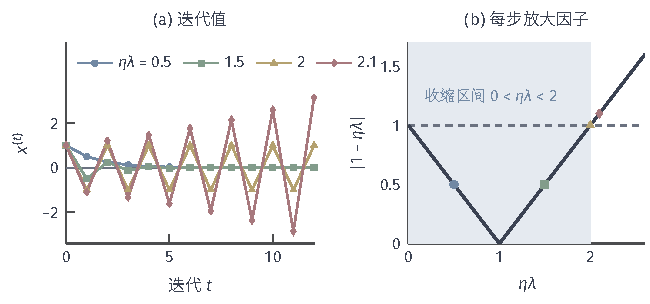
\includegraphics[width=110.0mm]{figures/03-optimization-evolution-and-signals/01-optimization/tikz/c3-step-size/figure.pdf}
  \caption{一维二次目标$f(x)=\lambda x^2/2$上的固定步长梯度下降，$x^{(0)}=1$。(a) 迭代值$x^{(t)}=(1-\eta\lambda)^t$，图例给出$\eta\lambda$；点只对应整数步，连线帮助追踪次序。(b) 每步的放大因子$|1-\eta\lambda|$，浅蓝区间$0<\eta\lambda<2$内因子小于$1$，四个彩色点对应(a)中的四个步长。}
  \label{fig:opt-smooth-step-size}
\end{figure}

\paragraph{共同例中的“之”字路径}
在二维共同例~\eqref{eq:opt-smooth-common-quadratic}上，两个坐标各自独立地按一维规律演化：$x_1$每步乘$1-\eta$，$x_2$每步乘$1-16\eta$。稳定要求$\eta<2/16=1/8$，由陡的$x_2$方向决定；而收敛快慢由最慢的因子决定。图~\ref{fig:opt-smooth-gd-zigzag}比较了三个步长。$\eta=1/16$时$x_2$一步归零，此后$x_1$每步只缩小到$15/16$；$\eta=2/17$使两个因子的绝对值相等，都是$15/17\approx0.882$，这是固定步长下的最佳折中，但$x_2$每步换号，路径在谷底两侧来回折返；$\eta=0.13$略超过$1/8$，$x_2$的因子为$-1.08$，路径越来越宽地横跨山谷，虽然$x_1$仍在收缩。一般地，对特征值在$[\mu,L]$中的正定二次目标，固定步长的最小最坏收缩因子是$(\kappa-1)/(\kappa+1)$，在$\eta=2/(L+\mu)$时取得；$\kappa$越大，路径越接近直线往返，收敛越慢。

\begin{figure*}[htbp]
  \centering
  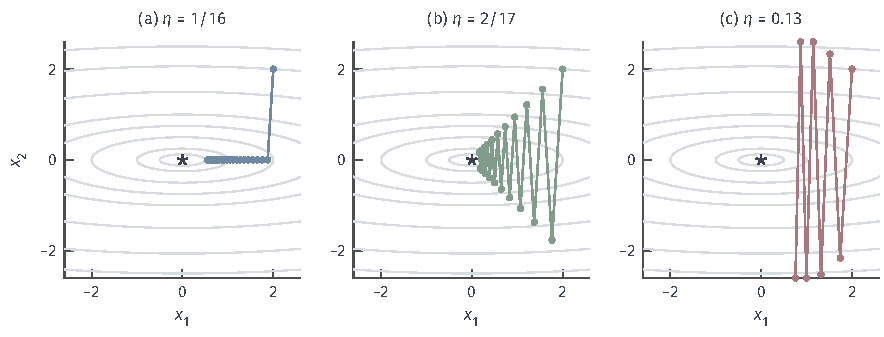
\includegraphics[width=149.7mm]{figures/03-optimization-evolution-and-signals/01-optimization/tikz/c3-gd-zigzag/figure.pdf}
  \caption{共同例$f(\bm x)=\tfrac12(x_1^2+16x_2^2)$上从$(2,2)^\top$出发的梯度下降路径，灰色椭圆是等高线，星号是最小点。(a) $\eta=1/16$：$x_2$一步消去，此后沿$x_1$轴缓慢前进（20步后$f\approx0.15$）。(b) $\eta=2/17$：两坐标因子为$\pm15/17$，路径呈“之”字。(c) $\eta=0.13>1/8$：$x_2$的因子为$-1.08$，路径越摆越宽（超出画面的点截在边框上）。}
  \label{fig:opt-smooth-gd-zigzag}
\end{figure*}

\paragraph{凸目标上的目标差}
若目标还是凸的，并且存在最小点，就可以从驻点残差推进到目标差。关键是把目标差和到最小点的距离联系起来。

\begin{theorem}[凸光滑目标上的梯度下降]
\label{thm:opt-smooth-gd-convex}
设$f$在$\mathbb R^d$上凸且$L$光滑，存在最小点$\bm x^\star$，取$\eta=1/L$。则对$T\geq1$，
\begin{equation}
\label{eq:opt-smooth-gd-convex-rate}
  f(\bm x^{(T)})-f^\star\leq\frac{L\lVert\bm x^{(0)}-\bm x^\star\rVert_2^2}{2T}.
\end{equation}
\end{theorem}

\begin{proof}
记$\bm g=\nabla f(\bm x)$，$\bm x^+=\bm x-\bm g/L$。由式~\eqref{eq:opt-smooth-gd-one-step}，$f(\bm x^+)\leq f(\bm x)-\lVert\bm g\rVert_2^2/(2L)$；由第~\ref{chap:optimization}章可微凸函数的一阶支撑下界，$f(\bm x)\leq f^\star+\langle\bm g,\bm x-\bm x^\star\rangle$。两式相加，再配方：
\[
  \begin{aligned}
  f(\bm x^+)-f^\star&\leq\langle\bm g,\bm x-\bm x^\star\rangle-\frac1{2L}\lVert\bm g\rVert_2^2\\
  &=\frac L2\Bigl(\lVert\bm x-\bm x^\star\rVert_2^2-\bigl\lVert\bm x-\bm x^\star-\tfrac1L\bm g\bigr\rVert_2^2\Bigr)\\
  &=\frac L2\bigl(\lVert\bm x-\bm x^\star\rVert_2^2-\lVert\bm x^+-\bm x^\star\rVert_2^2\bigr).
  \end{aligned}
\]
对$t=0,\dots,T-1$相加，右边相消为$\tfrac L2(\lVert\bm x^{(0)}-\bm x^\star\rVert_2^2-\lVert\bm x^{(T)}-\bm x^\star\rVert_2^2)\leq\tfrac L2\lVert\bm x^{(0)}-\bm x^\star\rVert_2^2$。左边是$\sum_{t=1}^{T}(f(\bm x^{(t)})-f^\star)$；目标值逐步不增，所以这个和不小于$T(f(\bm x^{(T)})-f^\star)$。
\end{proof}

证明顺带说明$\lVert\bm x^{(t)}-\bm x^\star\rVert_2$逐步不增：迭代点不会远离任何一个最小点。这个结论用到凸性；没有凸性时只有定理~\ref{thm:opt-smooth-gd-nonconvex}的残差保证。

\paragraph{回溯线搜索}
固定步长要求事先知道$L$。估计偏大则步长过小、进展缓慢；估计偏小则式~\eqref{eq:opt-smooth-gd-one-step}的系数可能为负，下降保证失效。另一种做法是不预先相信任何常数，而用实际函数值检验每一步：先试一个较大的步长，若目标没有“足够地”下降就缩小，直到下降为止。这里“足够”是指实际下降至少达到一阶预测的固定比例。设$\bm g\neq\bm0$，参数$c\in(0,1)$，\term{Armijo条件}（Armijo condition）要求
\begin{equation}
\label{eq:opt-smooth-armijo}
  f(\bm x-\eta\bm g)\leq f(\bm x)-c\,\eta\lVert\bm g\rVert_2^2 .
\end{equation}
右边是把切线的斜率打了折扣$c$的直线。按固定比例缩小步长直到满足它，称为\term{回溯线搜索}（backtracking line search），它是\term{线搜索}（line search）最常用的形式。

\begin{algorithm}[带回溯线搜索的一步梯度下降]
\label{alg:opt-smooth-backtracking}
\begin{algorithmic}[1]
\Require 当前点$\bm x$与梯度$\bm g=\nabla f(\bm x)\neq\bm0$，函数值$f(\bm x)$，初始试探步长$\bar\eta>0$，缩减比例$\gamma\in(0,1)$，参数$c\in(0,1)$
\Ensure 接受的步长$\eta$与新点$\bm x^+$
\State $\eta\gets\bar\eta$
\State 计算试探点$\bm x-\eta\bm g$的函数值
\While{$f(\bm x-\eta\bm g)>f(\bm x)-c\eta\lVert\bm g\rVert_2^2$}
  \State $\eta\gets\gamma\eta$ \Comment{拒绝试探点，缩短步长}
  \State 计算新试探点的函数值
\EndWhile
\State \Return $\eta$，$\bm x^+=\bm x-\eta\bm g$
\end{algorithmic}
\end{algorithm}

执行次序是：先算试探点的函数值，与右边的阈值比较；不满足就丢弃该点、缩短步长，再算下一个试探点。每次拒绝多花一次函数值计算，不需要新的梯度。若$\bm g=\bm0$，算法在线搜索之前已按驻点停止。

\begin{example}[共同例上的一次回溯]
\label{ex:opt-smooth-armijo}
在$\bm x^{(0)}=(2,2)^\top$处，$\bm g=(2,32)^\top$，$\lVert\bm g\rVert_2^2=1028$。取$\bar\eta=1$，$\gamma=1/2$，$c=1/4$，阈值为$34-257\eta$。依次试探：$\eta=1$时$f=7200$；$\eta=1/2$时$f=1568.5$；$\eta=1/4$时$f\approx289.1$；$\eta=1/8$时试探点为$(1.75,-2)^\top$，$f\approx33.53$，虽然低于$34$，却高于阈值$1.875$，仍被拒绝；$\eta=1/16$时试探点为$(1.875,0)^\top$，$f\approx1.758$，低于阈值$17.94$，接受。共计算了五次函数值、拒绝四次。图~\ref{fig:opt-smooth-armijo}画出最后两次试探：曲线$\varphi(\eta)=f(\bm x-\eta\bm g)$落在Armijo线下方的步长构成绿色区间。$\eta=1/8$被拒绝说明，“目标比原来低”还不够，Armijo条件要求下降与步长成比例。
\end{example}

\begin{figure}[htbp]
  \centering
  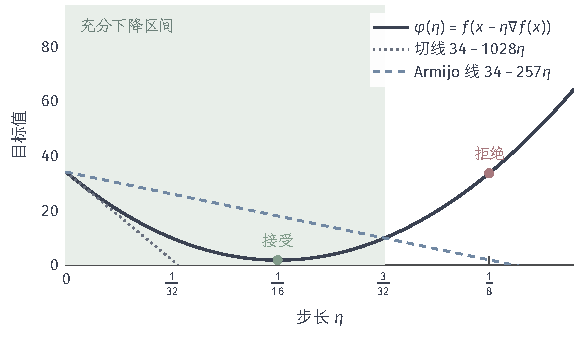
\includegraphics[width=98.0mm]{figures/03-optimization-evolution-and-signals/01-optimization/tikz/c3-armijo/figure.pdf}
  \caption{共同例在$\bm x=(2,2)^\top$处沿负梯度的一维截面$\varphi(\eta)=f(\bm x-\eta\nabla f(\bm x))$。点线是切线$34-1028\eta$，蓝色虚线是$c=1/4$的Armijo线$34-257\eta$，绿色区间是满足Armijo条件的步长。从$\bar\eta=1$开始减半，$\eta=1,\,1/2,\,1/4$的函数值远在画面之外，$\eta=1/8$（红点）虽使目标略降却在Armijo线之上被拒绝，$\eta=1/16$（绿点）被接受。}
  \label{fig:opt-smooth-armijo}
\end{figure}

\paragraph{回溯的有限结束与保证}
回溯的价值在于：它不需要知道$L$，但只要$L$存在，就一定有限步结束，且接受的步长不会太小。由式~\eqref{eq:opt-smooth-gd-one-step}，$\eta\leq2(1-c)/L$时$1-L\eta/2\geq c$，Armijo条件必然成立。因此当$f$为$L$光滑时，试探步长一旦落到$2(1-c)/L$以下就被接受，至多拒绝$\lceil\log_{1/\gamma}(\bar\eta L/(2(1-c)))\rceil$次（$\bar\eta\leq2(1-c)/L$时不拒绝），接受的步长满足
\[
  \eta\geq\eta_{\min}=\min\Bigl\{\bar\eta,\ \frac{2\gamma(1-c)}{L}\Bigr\}.
\]
例~\ref{ex:opt-smooth-armijo}中$2(1-c)/L=3/32$，实际接受的$1/16$确实不小于$\gamma\cdot3/32$。

每步下降至少$c\,\eta_{\min}\lVert\bm g^{(t)}\rVert_2^2$，按定理~\ref{thm:opt-smooth-gd-nonconvex}的证明累加，非凸情形得到$\min_{t<T}\lVert\nabla f(\bm x^{(t)})\rVert_2^2\leq(f(\bm x^{(0)})-f_{\inf})/(Tc\,\eta_{\min})$。凸情形若取$c=1/2$，接受的步长$\eta^{(t)}$满足$f(\bm x^{(t+1)})\leq f(\bm x^{(t)})-\tfrac{\eta^{(t)}}2\lVert\bm g^{(t)}\rVert_2^2$；把定理~\ref{thm:opt-smooth-gd-convex}证明中的$1/L$换成$\eta^{(t)}$，同样的配方给出
\[
  \eta^{(t)}\bigl(f(\bm x^{(t+1)})-f^\star\bigr)\leq\frac12\bigl(\lVert\bm x^{(t)}-\bm x^\star\rVert_2^2-\lVert\bm x^{(t+1)}-\bm x^\star\rVert_2^2\bigr),
\]
相加并利用目标单调与$\eta^{(t)}\geq\eta_{\min}$，得到$f(\bm x^{(T)})-f^\star\leq\lVert\bm x^{(0)}-\bm x^\star\rVert_2^2/(2T\eta_{\min})$，这里$\eta_{\min}=\min\{\bar\eta,\gamma/L\}$。这两条保证分别针对历史最佳残差点和最后一点，与固定步长的情形一致。回溯的代价是每轮多出的函数值计算；它不能弥补错误的梯度，也不能处理无下界的目标。

\subsection{预条件与坐标变换}
\label{sec:opt-smooth-preconditioning}

“之”字路径的根源是同一个标量步长要同时服务于曲率$1$和曲率$16$两个方向。若能对不同方向使用不同的步长，例如$x_1$方向走$1$、$x_2$方向走$1/16$，一步就能到达原点。本小节把这种想法写成固定的线性坐标变换。

\paragraph{固定预条件就是换坐标}
取固定的对称正定矩阵$\bm P$，更新
\begin{equation}
\label{eq:opt-smooth-preconditioned-gd}
  \bm x^{(t+1)}=\bm x^{(t)}-\eta\bm P\nabla f(\bm x^{(t)})
\end{equation}
称为\term{预条件}（preconditioning）梯度法，$\bm P$称为预条件矩阵。令$\bm x=\bm P^{1/2}\bm z$，定义$h(\bm z)=f(\bm P^{1/2}\bm z)$。由链式法则$\nabla h(\bm z)=\bm P^{1/2}\nabla f(\bm x)$，对$h$作普通梯度下降$\bm z^+=\bm z-\eta\nabla h(\bm z)$，两边左乘$\bm P^{1/2}$恰好得到式~\eqref{eq:opt-smooth-preconditioned-gd}。所以预条件梯度法就是在新坐标$\bm z$中的普通梯度下降：它不改变目标的值和最小点，只改变“哪个方向算作一步”。新坐标中的Hessian是
\[
  \nabla^2h(\bm z)=\bm P^{1/2}\,\nabla^2f(\bm x)\,\bm P^{1/2},
\]
它与$\bm P\nabla^2f(\bm x)$相似，因而特征值相同。对正定二次目标$\tfrac12\bm x^\top\bm H\bm x$，上一小节的全部结论在$\bm z$坐标中成立：收敛当且仅当$0<\eta<2/\lambda_{\max}(\bm P^{1/2}\bm H\bm P^{1/2})$，最佳固定步长的收缩因子为$(\tilde\kappa-1)/(\tilde\kappa+1)$，其中$\tilde\kappa$是变换后Hessian的条件数。

\begin{example}[共同例上的两个预条件]
\label{ex:opt-smooth-preconditioning}
取$\bm P=\operatorname{diag}(1,1/16)$，则$\bm P\nabla f(\bm x)=\bm x$，变换后Hessian为$\bm I$，$\tilde\kappa=1$。取$\eta=1/2$，每步$\bm x^{(t+1)}=\bm x^{(t)}/2$，迭代沿对角线直奔原点；取$\eta=1$则一步到达。反过来取$\bm P=\operatorname{diag}(1/16,1)$，它的条件数同样是$16$，变换后Hessian却是$\operatorname{diag}(1/16,16)$，条件数$256$，最佳固定步长的收缩因子从$15/17\approx0.882$恶化到$255/257\approx0.992$。图~\ref{fig:opt-smooth-preconditioning}在三个坐标系中画出这三种情形：在合适的$\bm z$坐标中，椭圆等高线变成圆，负梯度直接指向圆心；在不合适的坐标中，椭圆反而被拉得更扁。
\end{example}

\begin{figure*}[htbp]
  \centering
  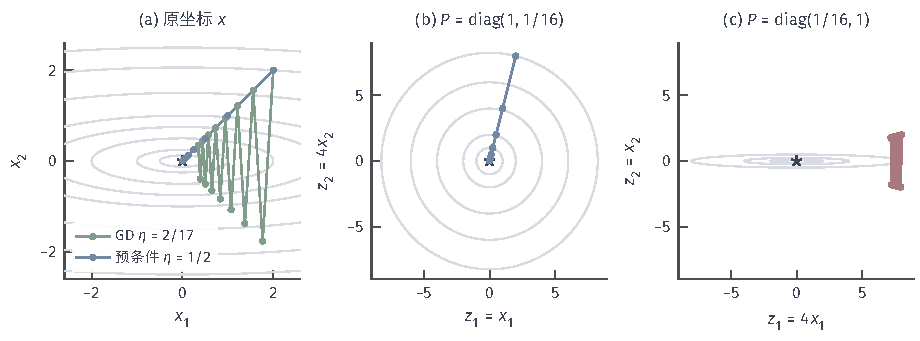
\includegraphics[width=155.7mm]{figures/03-optimization-evolution-and-signals/01-optimization/tikz/c3-preconditioning/figure.pdf}
  \caption{固定预条件作为坐标变换。(a) 原坐标中，普通梯度下降（绿，$\eta=2/17$）走“之”字，$\bm P=\operatorname{diag}(1,1/16)$、$\eta=1/2$的预条件更新（蓝）每步把$\bm x$减半，沿直线到达原点。(b) 在$\bm z=\bm P^{-1/2}\bm x=(x_1,4x_2)$坐标中，等高线是圆，蓝色路径就是普通梯度下降。(c) 若取$\bm P=\operatorname{diag}(1/16,1)$，$\bm z=(4x_1,x_2)$，变换后Hessian为$\operatorname{diag}(1/16,16)$，等高线更扁；红色是此坐标中最佳固定步长$\eta=2/(16+1/16)$的14步，每步横跨山谷，沿长轴几乎不动。}
  \label{fig:opt-smooth-preconditioning}
\end{figure*}

例子说明，判断预条件好坏的标准是变换后的曲率$\bm P^{1/2}\bm H\bm P^{1/2}$，而不是$\bm P$自身的条件数。理想的$\bm P$是$\bm H^{-1}$，但求它等于解原问题；实际的预条件在“变换后曲率接近常数倍单位阵”与“构造和应用$\bm P$的成本”之间折中。对角$\bm P$每轮只多$O(d)$次乘法，稠密$\bm P$需要$O(d^2)$存储与每轮$O(d^2)$运算，若$\bm P$以分解形式给出，成本取决于分解结构。本小节的分析要求$\bm P$在迭代中固定；按历史梯度统计逐轮改变的缩放，其构造、正定性与收敛分析在第~\ref{chap:opt-stochastic-block}章讨论。

\paragraph{选定度量中的最陡下降}
预条件还有另一种读法：它改变了“最陡”的含义。给定对称正定矩阵$\bm M$，定义范数$\lVert\bm v\rVert_{\bm M}=\sqrt{\bm v^\top\bm M\bm v}$。在单位$\bm M$-球上使方向导数最小的方向，称为该度量下的\term{最陡下降方向}（steepest descent direction）。由$\bm M$-内积的Cauchy--Schwarz不等式，
\[
  \langle\bm g,\bm d\rangle=(\bm M^{-1}\bm g)^\top\bm M\bm d\geq-\lVert\bm M^{-1}\bm g\rVert_{\bm M}\lVert\bm d\rVert_{\bm M},
\]
等号在$\bm d$与$-\bm M^{-1}\bm g$同向时取得，所以最陡下降方向是$-\bm M^{-1}\bm g/\lVert\bm M^{-1}\bm g\rVert_{\bm M}$。取$\bm M=\bm I$得到负梯度，取$\bm M=\bm P^{-1}$得到$-\bm P\bm g$的方向。负梯度只是欧氏度量下的最陡方向；同一个目标在不同度量下有不同的“最陡”方向。

换了度量，与之配套的光滑常数和残差也要一起换。若对所有$\bm x,\bm p$有$f(\bm x+\bm p)\leq f(\bm x)+\langle\bm g,\bm p\rangle+\tfrac{L_{\bm M}}2\lVert\bm p\rVert_{\bm M}^2$，把$\bm p=-\eta\bm M^{-1}\bm g$代入，与式~\eqref{eq:opt-smooth-gd-one-step}同样的推导给出
\[
  f(\bm x^+)\leq f(\bm x)-\eta\Bigl(1-\frac{L_{\bm M}\eta}2\Bigr)\bm g^\top\bm M^{-1}\bm g .
\]
步长上限由$L_{\bm M}$决定，衡量进展的残差是$\sqrt{\bm g^\top\bm M^{-1}\bm g}$，而不再是$\lVert\bm g\rVert_2$。共同例取$\bm M=\operatorname{diag}(1,16)$时$L_{\bm M}=1$，残差$\sqrt{g_1^2+g_2^2/16}$；用欧氏残差$\lVert\bm g\rVert_2$作停止判据，同样的容差在两个坐标方向上就对应了相差$16$倍的精度要求。本章只用固定的正定度量；由概率模型诱导的Fisher度量与自然梯度属于分布几何，可参考\BookChapterRef{chap:information-theory-and-statistical-geometry}{卷四“概率分布的分析与优化”章}。

\subsection{重球动量法}
\label{sec:opt-smooth-heavy-ball}

预条件需要事先知道各方向的曲率。另一种思路不改坐标，而让更新记住前一步的位移。观察图~\ref{fig:opt-smooth-gd-zigzag}(b)：连续两步在$x_2$方向上符号相反，在$x_1$方向上符号相同。若把上一步的位移按比例叠加到这一步，横跨山谷的分量相互抵消，沿谷底的分量逐步累积，就像一个有惯性的小球沿槽滚下，而不是每步都重新起跑。

\paragraph{状态与一轮更新}
\term{重球法}（heavy-ball method）是经典的\term{动量法}（momentum method）\cite{polyak1964heavyball}，它的更新为
\begin{equation}
\label{eq:opt-smooth-heavy-ball}
  \bm x^{(t+1)}=\bm x^{(t)}-\eta\nabla f(\bm x^{(t)})+\beta\bigl(\bm x^{(t)}-\bm x^{(t-1)}\bigr),\qquad 0\leq\beta<1 .
\end{equation}
算法的完整状态是一对点$(\bm x^{(t)},\bm x^{(t-1)})$，等价地是当前点与上一步位移；只知道$\bm x^{(t)}$无法继续迭代。约定$\bm x^{(-1)}=\bm x^{(0)}$，即零动量启动，第一步就是普通梯度步。每轮仍只算一次梯度，额外的代价是存储一个向量和几次向量加法。$\beta=0$时退回梯度下降。

\paragraph{二次目标上的逐方向递推}
在正定二次目标$f(\bm x)=\tfrac12(\bm x-\bm x^\star)^\top\bm H(\bm x-\bm x^\star)$上，误差$\bm e^{(t)}=\bm x^{(t)}-\bm x^\star$满足$\bm e^{(t+1)}=(\bm I-\eta\bm H)\bm e^{(t)}+\beta(\bm e^{(t)}-\bm e^{(t-1)})$。在$\bm H$的特征向量基下各分量互不耦合，曲率为$\lambda$的分量满足二阶线性递推
\begin{equation}
\label{eq:opt-smooth-hb-recursion}
  e^{(t+1)}=(1+\beta-\eta\lambda)\,e^{(t)}-\beta\,e^{(t-1)} .
\end{equation}
它的解是特征方程$r^2-(1+\beta-\eta\lambda)r+\beta=0$两根的幂的组合（重根时还有$t\,r^t$项），所以收敛快慢由较大的根模决定。与梯度下降的一阶递推$e^{(t+1)}=(1-\eta\lambda)e^{(t)}$相比，多出的一项$-\beta e^{(t-1)}$使误差能以阻尼振荡的方式衰减：两根为共轭复数时，模都等于$\sqrt\beta$，与$\lambda$无关。

\paragraph{稳定范围与参数选择}
两根都在单位圆内的条件，可以由二次多项式$r^2+a_1r+a_0$的判据$|a_0|<1$、$|a_1|<1+a_0$读出：这里$a_0=\beta$、$a_1=-(1+\beta-\eta\lambda)$，条件化为
\[
  0<\eta\lambda<2(1+\beta).
\]
动量把稳定的步长上界从$2/L$放宽到$2(1+\beta)/L$。根为复数当且仅当$(1+\beta-\eta\lambda)^2<4\beta$，即$(1-\sqrt\beta)^2<\eta\lambda<(1+\sqrt\beta)^2$，此时根模恰为$\sqrt\beta$。若谱区间$[\mu,L]$已知，选$\eta,\beta$使$\eta\mu=(1-\sqrt\beta)^2$、$\eta L=(1+\sqrt\beta)^2$，整个区间都落在复根区（端点为重根），解得
\begin{equation}
\label{eq:opt-smooth-hb-parameters}
  \eta=\frac{4}{(\sqrt L+\sqrt\mu)^2},\qquad
  \beta=\Bigl(\frac{\sqrt L-\sqrt\mu}{\sqrt L+\sqrt\mu}\Bigr)^2,\qquad
  \sqrt\beta=\frac{\sqrt\kappa-1}{\sqrt\kappa+1}.
\end{equation}
每个方向的根模都不超过$\sqrt\beta$，端点处重根带来的$t\,r^t$因子只使衰减慢一个多项式倍数。共同例中$\kappa=16$，得$\eta=4/25$、$\beta=9/25$、$\sqrt\beta=3/5$，而梯度下降的最佳因子是$15/17\approx0.882$。达到同一误差所需的轮数大约正比于$1/(1-\text{因子})$，前者约$\sqrt\kappa/2$、后者约$\kappa/2$，这就是“加速”一词的含义。

图~\ref{fig:opt-smooth-momentum-stability}画出最大根模随$\eta\lambda$的变化。$\beta=9/25$的曲线在浅蓝区间$[\eta\mu,\eta L]=[0.16,2.56]$上平坦地等于$0.6$；$\beta=0$即梯度下降，曲线是折线$|1-\eta\lambda|$，只在$\eta\lambda=1$附近较低；$\beta=0.81$的稳定范围更宽（到$3.62$），平坦部分却抬高到$0.9$。动量过大并不会立即发散，而是让误差以接近$1$的模长期振荡；$\eta\lambda$超过$2(1+\beta)$时则一定发散。

\begin{figure}[htbp]
  \centering
  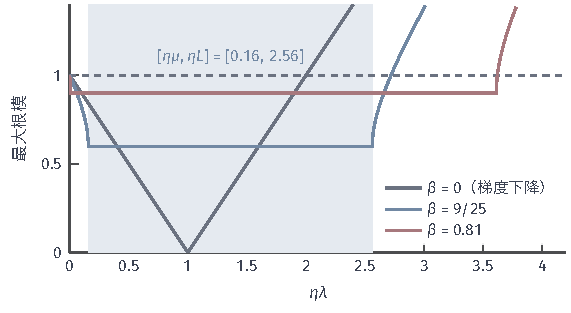
\includegraphics[width=96.6mm]{figures/03-optimization-evolution-and-signals/01-optimization/tikz/c3-momentum-stability/figure.pdf}
  \caption{重球法递推~\eqref{eq:opt-smooth-hb-recursion}的最大根模与$\eta\lambda$的关系（大于$1.4$的部分截去）。灰线$\beta=0$即梯度下降；蓝线$\beta=9/25$对应共同例的参数~\eqref{eq:opt-smooth-hb-parameters}，在浅蓝区间$[\eta\mu,\eta L]=[0.16,2.56]$上恒为$0.6$；红线$\beta=0.81$在复根区恒为$0.9$。虚线是稳定边界$1$。}
  \label{fig:opt-smooth-momentum-stability}
\end{figure}

\paragraph{结论的范围}
动量使目标值不再逐步单调。在共同例上用参数~\eqref{eq:opt-smooth-hb-parameters}，第一步是步长$4/25$的普通梯度步，这个步长超过了梯度下降的稳定上界$1/8$：$\bm x^{(1)}=(1.68,-3.12)^\top$，目标从$34$升到约$79.29$；此后惯性项开始抵消横向摆动，图~\ref{fig:opt-smooth-momentum-paths}中的蓝色曲线在第$10$步前后降到梯度下降之下。以上稳定范围和速率都是在正定二次目标、已知谱界的条件下逐方向算出的。对一般强凸光滑目标，重球法用这组参数并不保证全局收敛；对非凸目标，二次例的加速结论更不能直接继承。实际使用动量时，停止判据仍应检查原目标的梯度范数，而不是位移或动量的大小。

\subsection{Nesterov加速梯度法}
\label{sec:opt-smooth-nesterov}

重球法在当前点求梯度，再叠加惯性；它的加速分析依赖二次目标的逐方向分解。Nesterov提出的做法改变了求梯度的位置：先沿惯性方向外推到一个前瞻点，在那里求梯度并走一步。这一改动使加速结论能够推广到一般的凸光滑目标\cite{nesterov1983method}。

\paragraph{三个点与一轮更新}
\term{Nesterov加速梯度}（Nesterov accelerated gradient）区分三类点：记录点$\bm x^{(t)}$，外推得到的前瞻点$\bm y^{(t)}$，以及在$\bm y^{(t)}$处求得的梯度。下面是凸、$L$光滑目标的一个版本\cite{beck2009fista}。

\begin{algorithm}[Nesterov加速梯度法]
\label{alg:opt-smooth-nesterov}
\begin{algorithmic}[1]
\Require $L$光滑凸目标$f$，常数$L$，初值$\bm x^{(0)}$，轮数$T$
\Ensure 最后一点$\bm x^{(T)}$
\State $\bm y^{(0)}\gets\bm x^{(0)}$，$\theta^{(0)}\gets1$
\For{$t=0,1,\dots,T-1$}
  \State $\bm x^{(t+1)}\gets\bm y^{(t)}-\frac1L\nabla f(\bm y^{(t)})$ \Comment{在前瞻点求梯度}
  \State $\theta^{(t+1)}\gets\bigl(1+\sqrt{1+4(\theta^{(t)})^2}\bigr)/2$
  \State $\bm y^{(t+1)}\gets\bm x^{(t+1)}+\dfrac{\theta^{(t)}-1}{\theta^{(t+1)}}\bigl(\bm x^{(t+1)}-\bm x^{(t)}\bigr)$ \Comment{外推}
\EndFor
\end{algorithmic}
\end{algorithm}

把更新写成与重球法相同的形状，记$\beta^{(t)}=(\theta^{(t-1)}-1)/\theta^{(t)}$（$t\geq1$，$\beta^{(0)}=0$），则
\[
  \text{重球法：}\ \bm x^{(t+1)}=\bm x^{(t)}+\beta(\bm x^{(t)}-\bm x^{(t-1)})-\eta\nabla f(\bm x^{(t)}),
\]
\[
  \text{Nesterov：}\ \bm x^{(t+1)}=\bm x^{(t)}+\beta^{(t)}(\bm x^{(t)}-\bm x^{(t-1)})-\tfrac1L\nabla f\bigl(\bm x^{(t)}+\beta^{(t)}(\bm x^{(t)}-\bm x^{(t-1)})\bigr).
\]
两者都把惯性项加到当前点上，区别只在梯度的求值位置：重球法在出发点求，Nesterov在惯性已经带到的位置求。若惯性把点带过了谷底，前瞻点处的梯度会把它拉回来，这是一种“提前修正”。另一个区别是$\beta^{(t)}$随$t$增大而趋于$1$，不需要知道$\mu$。每轮的代价仍是一次梯度和几次向量运算，状态是$(\bm x^{(t)},\bm x^{(t-1)},\theta^{(t)})$。

\paragraph{加速保证}
在凸、光滑、最小点存在的条件下，Nesterov方法的目标差以$1/T^2$的速度下降，而定理~\ref{thm:opt-smooth-gd-convex}给出的梯度下降保证是$1/T$。证明不比较相邻两步的目标值，而是构造一个把目标差与距离合在一起的量，即\term{势函数}（potential function），证明它逐步不增。

\begin{theorem}[Nesterov方法的收敛速度]
\label{thm:opt-smooth-nesterov}
设$f$在$\mathbb R^d$上凸且$L$光滑（$L>0$），存在最小点$\bm x^\star$。则算法~\ref{alg:opt-smooth-nesterov}的迭代满足
\begin{equation}
\label{eq:opt-smooth-nesterov-rate}
  f(\bm x^{(T)})-f^\star\leq\frac{2L\lVert\bm x^{(0)}-\bm x^\star\rVert_2^2}{(T+1)^2},\qquad T\geq1 .
\end{equation}
\end{theorem}

\begin{proof}
\emph{三点不等式。}对任意$\bm y$，令$\bm x^+=\bm y-\nabla f(\bm y)/L$。下降引理给$f(\bm x^+)\leq f(\bm y)-\lVert\nabla f(\bm y)\rVert_2^2/(2L)$，凸性给$f(\bm y)\leq f(\bm v)+\langle\nabla f(\bm y),\bm y-\bm v\rangle$对任意$\bm v$成立。相加后与定理~\ref{thm:opt-smooth-gd-convex}的证明一样配方，得
\begin{equation}
\label{eq:opt-smooth-three-point}
  f(\bm x^+)\leq f(\bm v)+\frac L2\bigl(\lVert\bm y-\bm v\rVert_2^2-\lVert\bm x^+-\bm v\rVert_2^2\bigr).
\end{equation}

\emph{选比较点。}记$\Delta^{(t)}=f(\bm x^{(t)})-f^\star$，$\theta=\theta^{(t)}$。在式~\eqref{eq:opt-smooth-three-point}中取$\bm y=\bm y^{(t)}$，$\bm v=(1-1/\theta)\bm x^{(t)}+\bm x^\star/\theta$。由$\theta\geq1$，$\bm v$是$\bm x^{(t)}$与$\bm x^\star$的凸组合，凸性给$f(\bm v)-f^\star\leq(1-1/\theta)\Delta^{(t)}$。引入辅助点$\bm u^{(t)}=\theta^{(t)}\bm y^{(t)}-(\theta^{(t)}-1)\bm x^{(t)}$，直接展开可得$\bm y^{(t)}-\bm v=(\bm u^{(t)}-\bm x^\star)/\theta$，以及$\bm x^{(t+1)}-\bm v=\bigl(\theta\bm x^{(t+1)}-(\theta-1)\bm x^{(t)}-\bm x^\star\bigr)/\theta$。把外推公式代入$\bm u^{(t+1)}$的定义：
\[
  \begin{aligned}
  \bm u^{(t+1)}&=\theta^{(t+1)}\bm x^{(t+1)}+(\theta^{(t)}-1)(\bm x^{(t+1)}-\bm x^{(t)})-(\theta^{(t+1)}-1)\bm x^{(t+1)}\\
  &=\theta^{(t)}\bm x^{(t+1)}-(\theta^{(t)}-1)\bm x^{(t)},
  \end{aligned}
\]
所以$\bm x^{(t+1)}-\bm v=(\bm u^{(t+1)}-\bm x^\star)/\theta$。于是式~\eqref{eq:opt-smooth-three-point}变为
\[
  \Delta^{(t+1)}\leq\Bigl(1-\frac1{\theta^{(t)}}\Bigr)\Delta^{(t)}+\frac{L}{2(\theta^{(t)})^2}\bigl(\lVert\bm u^{(t)}-\bm x^\star\rVert_2^2-\lVert\bm u^{(t+1)}-\bm x^\star\rVert_2^2\bigr).
\]

\emph{势函数不增。}两边乘$(\theta^{(t)})^2$。参数的更新式等价于$(\theta^{(t)})^2-\theta^{(t)}=(\theta^{(t-1)})^2$（$t\geq1$），而$\theta^{(0)}=1$使$(\theta^{(0)})^2-\theta^{(0)}=0$。定义势函数
\[
  E^{(0)}=\frac L2\lVert\bm x^{(0)}-\bm x^\star\rVert_2^2,\qquad
  E^{(t)}=(\theta^{(t-1)})^2\Delta^{(t)}+\frac L2\lVert\bm u^{(t)}-\bm x^\star\rVert_2^2\quad(t\geq1),
\]
注意$\bm u^{(0)}=\bm x^{(0)}$，上式正是$E^{(t+1)}\leq E^{(t)}$，对所有$t\geq0$成立。因此$(\theta^{(T-1)})^2\Delta^{(T)}\leq E^{(T)}\leq E^{(0)}$。

\emph{参数的增长。}由$\theta^{(t+1)}=\bigl(1+\sqrt{1+4(\theta^{(t)})^2}\bigr)/2\geq(1+2\theta^{(t)})/2=\theta^{(t)}+1/2$及$\theta^{(0)}=1$，归纳得$\theta^{(t)}\geq(t+2)/2$。取$t=T-1$代入上一段即得式~\eqref{eq:opt-smooth-nesterov-rate}。
\end{proof}

证明中下降的是势函数$E^{(t)}$，而不是目标值本身。势函数的第二项会随迭代把“能量”转给第一项，所以目标值可以在某些步上升。图~\ref{fig:opt-smooth-momentum-paths}(b)中，Nesterov方法的目标差在共同例上呈阶梯状起伏，但始终位于绿色点线所示的上界$2L\lVert\bm x^{(0)}-\bm x^\star\rVert_2^2/(t+1)^2=256/(t+1)^2$之下。

\begin{figure*}[htbp]
  \centering
  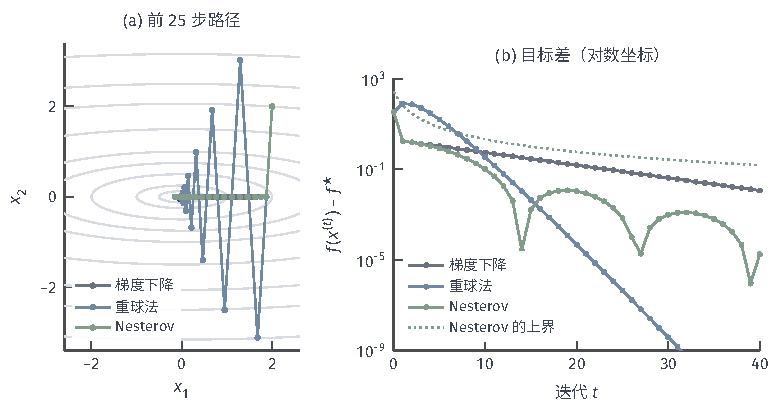
\includegraphics[width=132.0mm]{figures/03-optimization-evolution-and-signals/01-optimization/tikz/c3-momentum-paths/figure.pdf}
  \caption{共同例上梯度下降（灰，$\eta=1/16$）、重球法（蓝，$\eta=4/25$、$\beta=9/25$）与Nesterov方法（绿，$L=16$）的比较，均从$(2,2)^\top$出发、每轮一次梯度。(a) 前25步的路径；重球法第一步越到$(1.68,-3.12)^\top$，随后惯性抵消横向摆动。(b) 目标差的对数坐标曲线：重球法按约$0.6^{2t}$下降，梯度下降按$(15/16)^{2t}$下降，Nesterov方法的曲线不单调，但始终在点线所示的$O(1/t^2)$上界之下。}
  \label{fig:opt-smooth-momentum-paths}
\end{figure*}

\paragraph{使用时的边界}
共同例是强凸的，图中重球法用了已知的$\mu$而快于Nesterov方法的凸版本；若同样已知$\mu$，Nesterov方法也有常数动量$(\sqrt\kappa-1)/(\sqrt\kappa+1)$的强凸版本，这里不展开。定理~\ref{thm:opt-smooth-nesterov}要求精确梯度、步长$1/L$与凸性；$L$未知时，回溯必须与加速方案的势函数配套设计，不能把算法~\ref{alg:opt-smooth-backtracking}直接套上。实现中常加入\emph{重启}：当目标值上升或动量方向与梯度夹角变钝时，把$\theta$重置为$1$，以抑制振荡。重启是经验上有效的补充，在凸情形下并不改变定理的结论；对非凸目标，加速的速率保证不能无条件搬用，仍须以原目标的梯度残差作停止判据。
